% Options for packages loaded elsewhere
\PassOptionsToPackage{unicode}{hyperref}
\PassOptionsToPackage{hyphens}{url}
%
\documentclass[
]{book}
\usepackage{amsmath,amssymb}
\usepackage{iftex}
\ifPDFTeX
  \usepackage[T1]{fontenc}
  \usepackage[utf8]{inputenc}
  \usepackage{textcomp} % provide euro and other symbols
\else % if luatex or xetex
  \usepackage{unicode-math} % this also loads fontspec
  \defaultfontfeatures{Scale=MatchLowercase}
  \defaultfontfeatures[\rmfamily]{Ligatures=TeX,Scale=1}
\fi
\usepackage{lmodern}
\ifPDFTeX\else
  % xetex/luatex font selection
\fi
% Use upquote if available, for straight quotes in verbatim environments
\IfFileExists{upquote.sty}{\usepackage{upquote}}{}
\IfFileExists{microtype.sty}{% use microtype if available
  \usepackage[]{microtype}
  \UseMicrotypeSet[protrusion]{basicmath} % disable protrusion for tt fonts
}{}
\makeatletter
\@ifundefined{KOMAClassName}{% if non-KOMA class
  \IfFileExists{parskip.sty}{%
    \usepackage{parskip}
  }{% else
    \setlength{\parindent}{0pt}
    \setlength{\parskip}{6pt plus 2pt minus 1pt}}
}{% if KOMA class
  \KOMAoptions{parskip=half}}
\makeatother
\usepackage{xcolor}
\usepackage{longtable,booktabs,array}
\usepackage{calc} % for calculating minipage widths
% Correct order of tables after \paragraph or \subparagraph
\usepackage{etoolbox}
\makeatletter
\patchcmd\longtable{\par}{\if@noskipsec\mbox{}\fi\par}{}{}
\makeatother
% Allow footnotes in longtable head/foot
\IfFileExists{footnotehyper.sty}{\usepackage{footnotehyper}}{\usepackage{footnote}}
\makesavenoteenv{longtable}
\usepackage{graphicx}
\makeatletter
\def\maxwidth{\ifdim\Gin@nat@width>\linewidth\linewidth\else\Gin@nat@width\fi}
\def\maxheight{\ifdim\Gin@nat@height>\textheight\textheight\else\Gin@nat@height\fi}
\makeatother
% Scale images if necessary, so that they will not overflow the page
% margins by default, and it is still possible to overwrite the defaults
% using explicit options in \includegraphics[width, height, ...]{}
\setkeys{Gin}{width=\maxwidth,height=\maxheight,keepaspectratio}
% Set default figure placement to htbp
\makeatletter
\def\fps@figure{htbp}
\makeatother
\setlength{\emergencystretch}{3em} % prevent overfull lines
\providecommand{\tightlist}{%
  \setlength{\itemsep}{0pt}\setlength{\parskip}{0pt}}
\setcounter{secnumdepth}{5}
\usepackage{booktabs}
\usepackage{amsthm}
\makeatletter
\def\thm@space@setup{%
  \thm@preskip=8pt plus 2pt minus 4pt
  \thm@postskip=\thm@preskip
}
\makeatother
\ifLuaTeX
  \usepackage{selnolig}  % disable illegal ligatures
\fi
\usepackage[]{natbib}
\bibliographystyle{apalike}
\IfFileExists{bookmark.sty}{\usepackage{bookmark}}{\usepackage{hyperref}}
\IfFileExists{xurl.sty}{\usepackage{xurl}}{} % add URL line breaks if available
\urlstyle{same}
\hypersetup{
  pdftitle={AI Tools in the Job Recruiting Process},
  pdfauthor={Jingyi (Vera) Wang, Kuigang (KG) Zhang, Michael Czapp, Xinqian (Demi) Dai, Yousuf Altameemi},
  hidelinks,
  pdfcreator={LaTeX via pandoc}}

\title{AI Tools in the Job Recruiting Process}
\author{Jingyi (Vera) Wang, Kuigang (KG) Zhang, Michael Czapp, Xinqian (Demi) Dai, Yousuf Altameemi}
\date{2023-07-31}

\begin{document}
\maketitle

{
\setcounter{tocdepth}{1}
\tableofcontents
}
\hypertarget{introduction-to-our-book}{%
\chapter{Introduction to Our Book}\label{introduction-to-our-book}}

For students at the Stephen M. Ross School of Business, the primary goal by graduation is to have a full-time job offer at a company and location that makes them excited to start their professional careers. Throughout the fall and winter semesters, recruiting is an incredibly time-consuming and stressful process, so students must use their time and effort efficiently to maximize their job opportunities. However, the recent and rapid progression of artificial intelligence (AI) tools has reshaped the recruiting landscape. Therefore, students need to understand how they can use these tools to their advantage and how recruiters may be using AI throughout the recruitment process.

Our book will provide a comprehensive overview of these AI tools. We will approach this from two perspectives: students' and recruiters'. For students, we discuss how they can use AI job finders, resume and cover letter optimization, practice interviews, and automated applications to support their professional endeavors. On the other hand, we discuss what AI tools recruiters may use, like applicant tracking systems (ATS), resume and cover letter screening, interview assessments, skill assessments, and predictive analytics. Then, we suggest how students should tailor their presentation of themselves to fit what these AI tools look for.

\hypertarget{about-us}{%
\chapter{About Us}\label{about-us}}

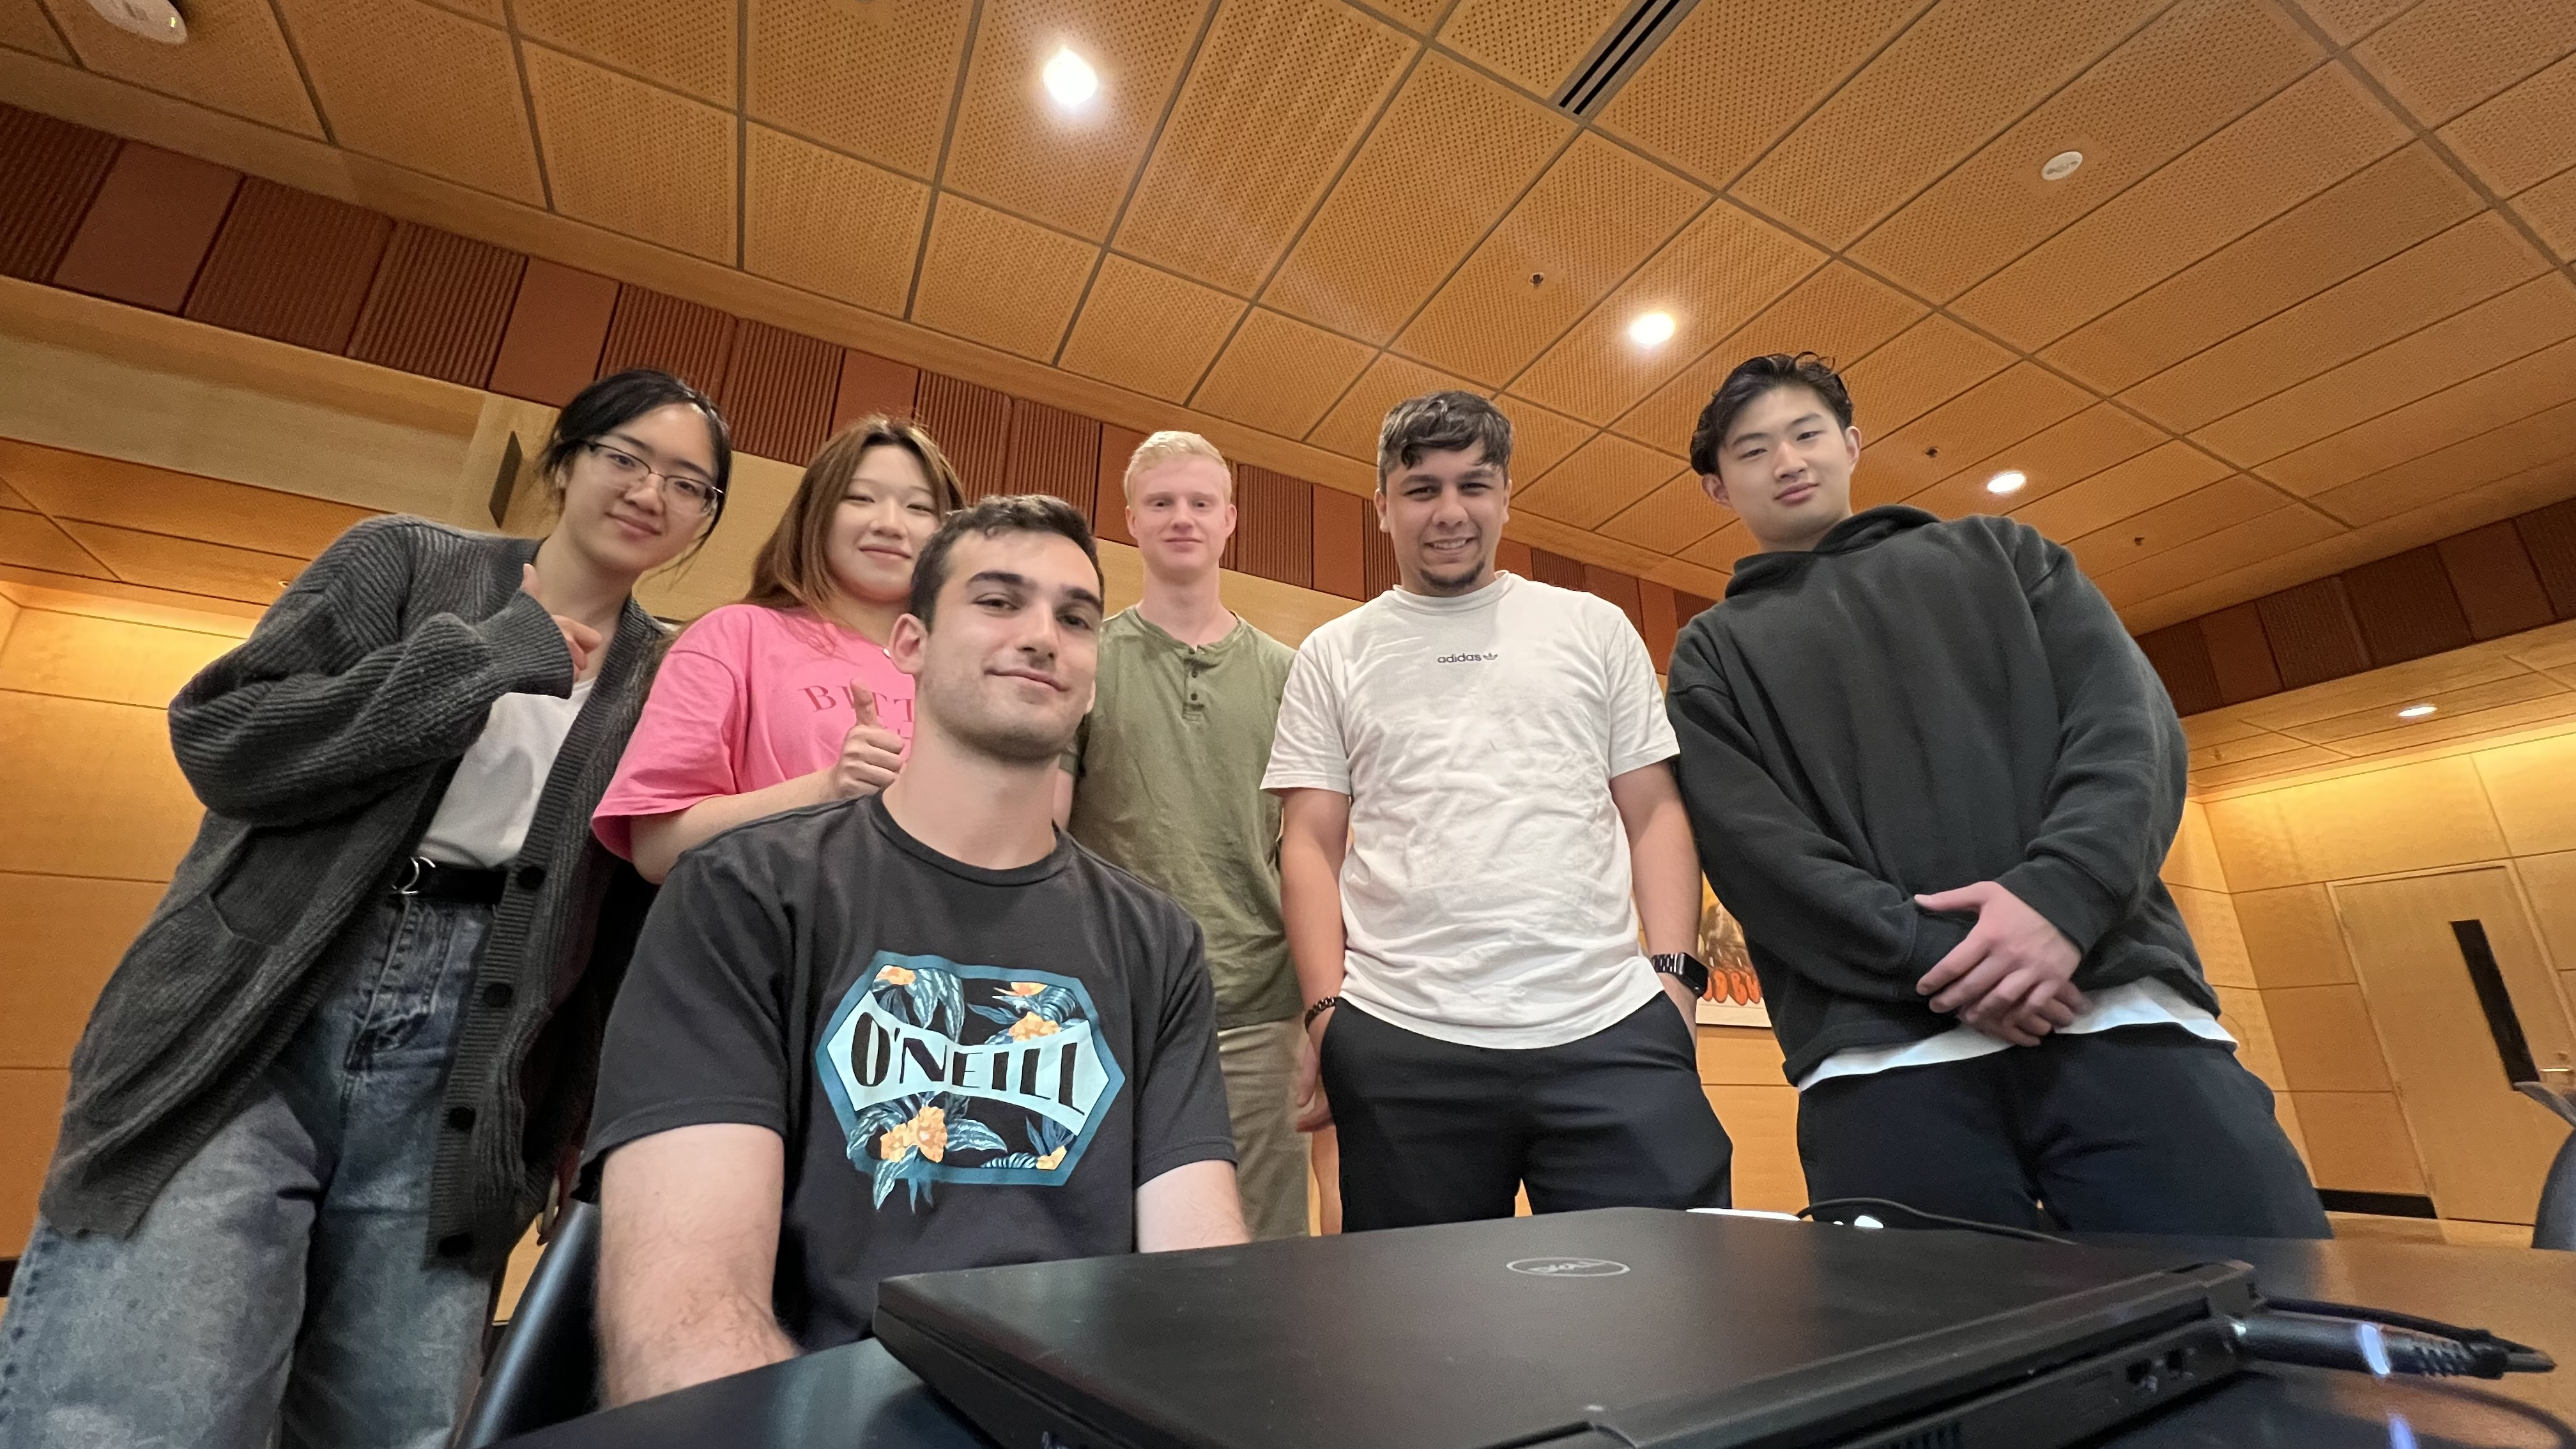
\includegraphics[width=4.04167in,height=\textheight]{Team Photo.jpg}

Our team, \textbf{Team Steve}, is driven by Steve's desire for a website that describes how new AI Tools are used in the recruitment process. For context, Steve (as seen in the black O'Neill shirt in the front left) is a student here at the Stephen M. Ross School of Business who is NOT in our project team. When deciding our team name, we thought it'd be a great idea to name it after the first person we encounter. We happened to run into Steve outside of our classroom, and the rest is history.

\hypertarget{jingyi-wang}{%
\section{Jingyi Wang}\label{jingyi-wang}}

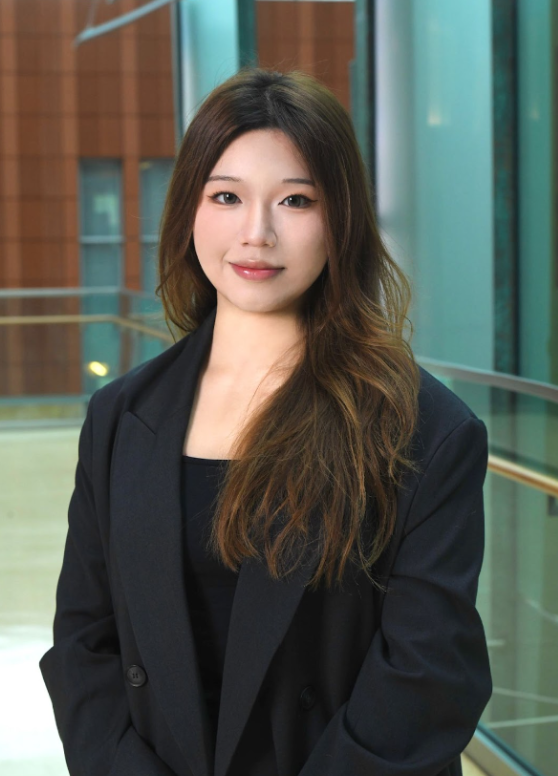
\includegraphics[width=2.16667in,height=\textheight]{Vera Photo.png}

\textbf{Background}

My name is Jingyi (Vera) Wang, currently a Master of Business Analytics student at the University of Michigan Ross School of Business. In May 2023, I graduated from Boston University with a concentration in Finance and Business Analytics. From my previous academic and internship experiences, I found my passion for business analytics. That's the reason why I decided to pursue a graduate degree in order to help me specialize in my area of interest and enrich my experience and knowledge in the field.

\textbf{Experience}

My experience is mainly composed of internships, projects, and case competitions. In 2021, I interned at Accenture as a management consulting intern. I managed project plans, conducted data analysis, and facilitated platform testing sessions for clients to improve the efficiency and accuracy of their online platform. In 2022, I interned at Vantage House Media as a finance intern. I generated comprehensive financial reports and provided stakeholders with valuable recommendations and potential VC prospects based on data analysis. In addition, I was a quantitative financial analyst intern at Shenwan Hongyuan Securities, where I built python models to select top-performing stocks and assess fund managers' performance.~

\textbf{Fun Facts}

\begin{itemize}
\item
  I have two pet guinea pigs
\item
  I never watch horror movies
\item
  I love photography, and I have previously operated a photography social account of my own
\end{itemize}

\hypertarget{kuigang-zhang}{%
\section{Kuigang Zhang}\label{kuigang-zhang}}

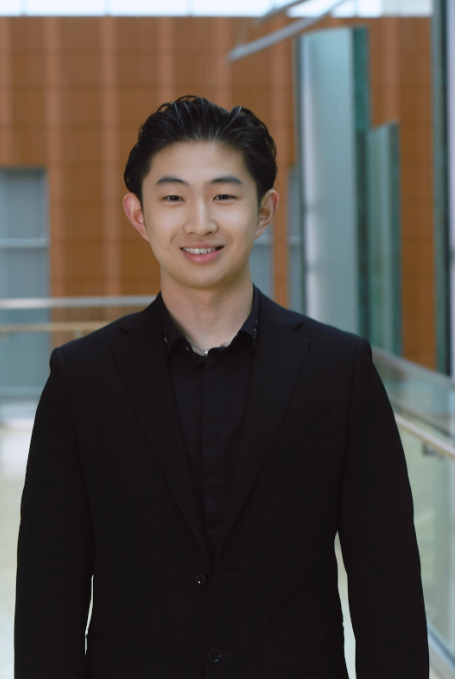
\includegraphics[width=2.1875in,height=\textheight]{KG Photo.png}

\textbf{Background}

My name is Kuigang Zhang, and I go by KG. I graduated from UCLA with a Data Science major and an Accounting minor in June 2023. Programming and business have been two areas that I am passionate about; therefore, I decided to pursue a Master of Business Analytics here at the University of Michigan Ross School of Business. I look forward to enriching my toolbox, meeting like-minded people, and getting the most out of the program.

\textbf{Experience}

I have four years of experience in programming, and have completed a number of Kaggle Competition as well as machine learning projects, and I have worked as an data analyst intern at the Shanghai Research Institute of Building Science Academy, where I enabled household energy consumption forecast in Shanghai for managing and planning urban energy utilization, covering a wide range of locations and building types.I have also worked as a data analyst intern at Lin Zhen Trading, where I developed an integrated data-driven retail supply chain management app in support of the bedding items business.

\textbf{Fun Facts}

\begin{itemize}
\item
  I was born and raised in Africa
\item
  I deadlift 400lbs
\item
  I speak 5 languages
\end{itemize}

\hypertarget{michael-czapp}{%
\section{Michael Czapp}\label{michael-czapp}}

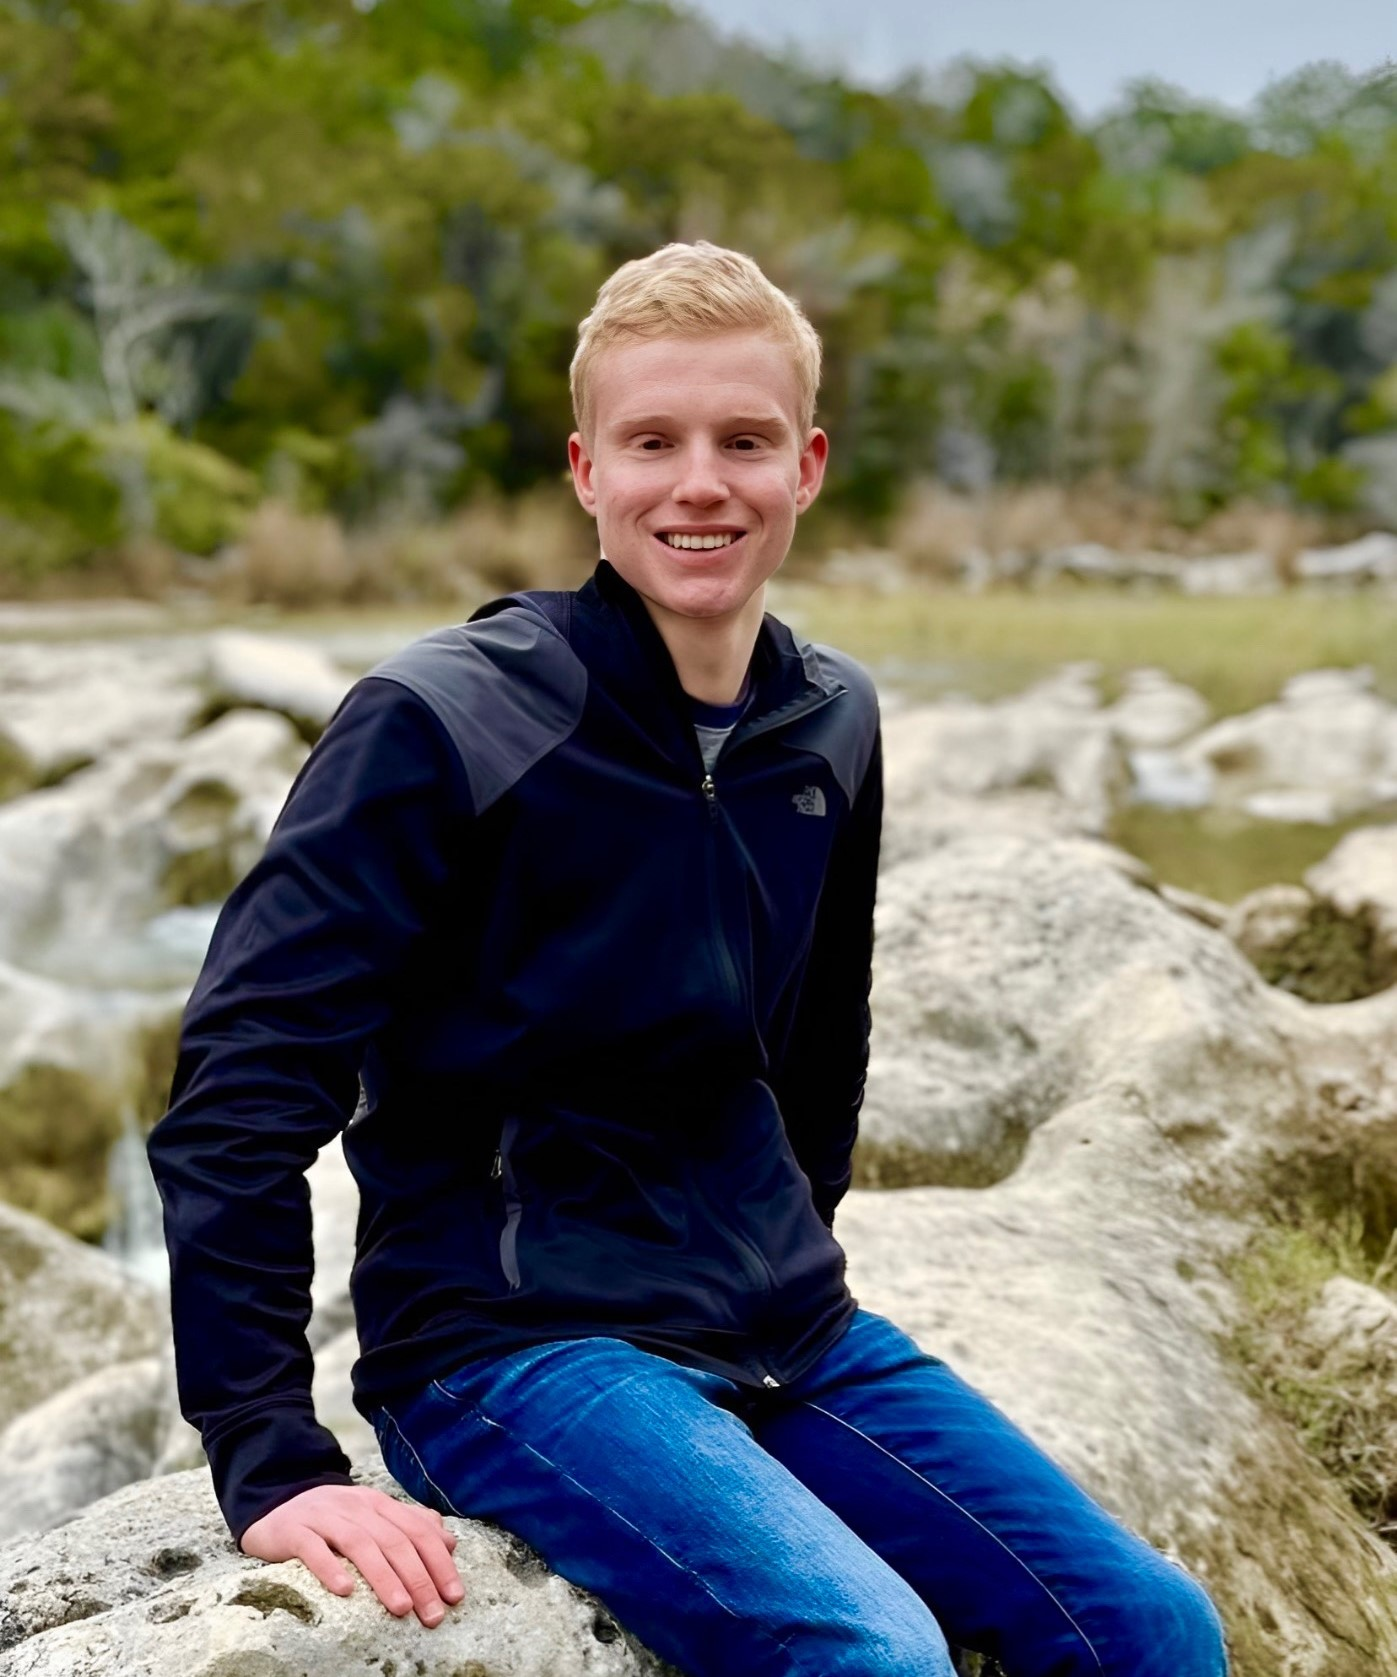
\includegraphics[width=2.36458in,height=\textheight]{Michael Czapp Photo.jpeg}

\textbf{Background}

My name is Michael Czapp, and I am currently a Master of Business Analytics (MBAn) student at the University of Michigan Ross School of Business. In April 2023, I graduated from the College of Engineering here with a Bachelor of Science in Industrial \& Operations Engineering. I knew I wanted to specialize in analytics, so starting a graduate program right after graduation made the most sense. It also allowed me to have an extra year at the University of Michigan and stay in my home state, and I plan to make the most of it!

\textbf{Experience}

My experience primarily consists of two summer internships. In 2021, I interned at DTE Energy in Detroit, MI as a Continuous Improvement Intern. I got to develop Power BI dashboards, lead a time study analysis on claim investigations, and support the execution of a pilot study at one of the company's sites. In 2022, I interned at Boston Scientific Corporation as a Global Supply Chain Consulting Intern, which was essentially an internal consulting role. I built automations, helped plan a global virtual conference, and used Excel to identify opportunities to decrease shipping costs to customers, all of which provided me with great experience in using data to discover meaningful insights to share with stakeholders.

\textbf{Fun Facts}

\begin{itemize}
\item
  Both my older brother and sister studied industrial engineering in undergrad
\item
  I play hockey as both a goalie and a skater
\item
  I've lived in the state of Michigan for my entire life
\end{itemize}

\hypertarget{xinqian-dai}{%
\section{Xinqian Dai}\label{xinqian-dai}}

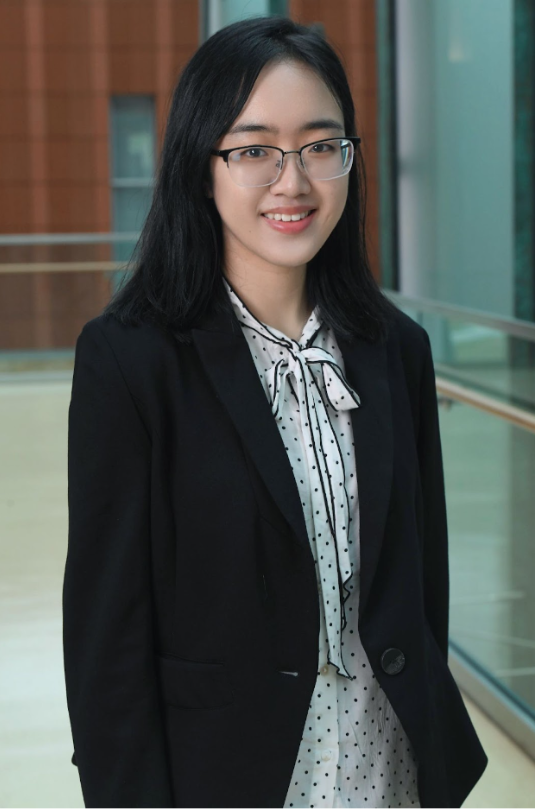
\includegraphics[width=2.08333in,height=\textheight]{Demi Photo.png}

\textbf{Background}

Hello! My name is Xinqian (Demi) Dai, and I come from the beautiful province of Heilongjiang, China, where I was born and raised. In 2019, I embarked on my exciting journey by enrolling at the University of Massachusetts Amherst for my undergraduate studies. I graduated with a double major in Marketing and Statistics in May 2023. My interest in Marketing has deep roots that extend back to my childhood days when I found myself more fascinated by the commercial inserts of a washing powder than the animated series on TV.~ Currently, I am intrigued by Customer Analytics, Advertising Effectiveness, and Digital Marketing, and I'm eager to delve deeper into these areas. Looking ahead, my post-graduation aspirations involve entering into the MarTech (Marketing Technology) industry. Armed with the knowledge and skills from the MBAn program, I aim to make a significant impact by applying data-driven strategies and innovative marketing technologies.

\textbf{Experience}

During my time at UMass Amherst, I engaged in a diverse range of research experiences and marketing projects. As a Marketing Research Assistant at the UMass Ombuds Office, I analyzed data from over 300 undergraduate student visitors, studying variables like gender and major to identify successful conflict resolution strategies. Utilizing R and Python, I applied regression models to estimate meeting times and understand the impact of visitor demographics on appointment durations. During my participation in the Research Experiences for Undergraduates (REU) Program, I conducted full-time research on Bayesian parameter estimations, highlighting the effectiveness of Bayesian models over traditional linear regression models. Additionally, as a Research Assistant in the UMass Marketing Department, I analyzed customer reactions to visual advertisements for various product categories and conducted experiments to evaluate the effect of different headbands on students. As a Strategist for the UMass AdLab, I designed customized questionnaires and implemented successful advertising strategies, resulting in a significant increase in orders for local companies. These experiences have shaped my passion for business analytics and my dedication to data-driven research and strategic planning.

\textbf{Fun Facts}

\begin{itemize}
\item
  A24 is my favorite film production company
\item
  I'm better at cooking than baking:))
\item
  My hometown holds the International Ice and Snow Festival every winter
\end{itemize}

\hypertarget{yousuf-altameemi}{%
\section{Yousuf Altameemi}\label{yousuf-altameemi}}

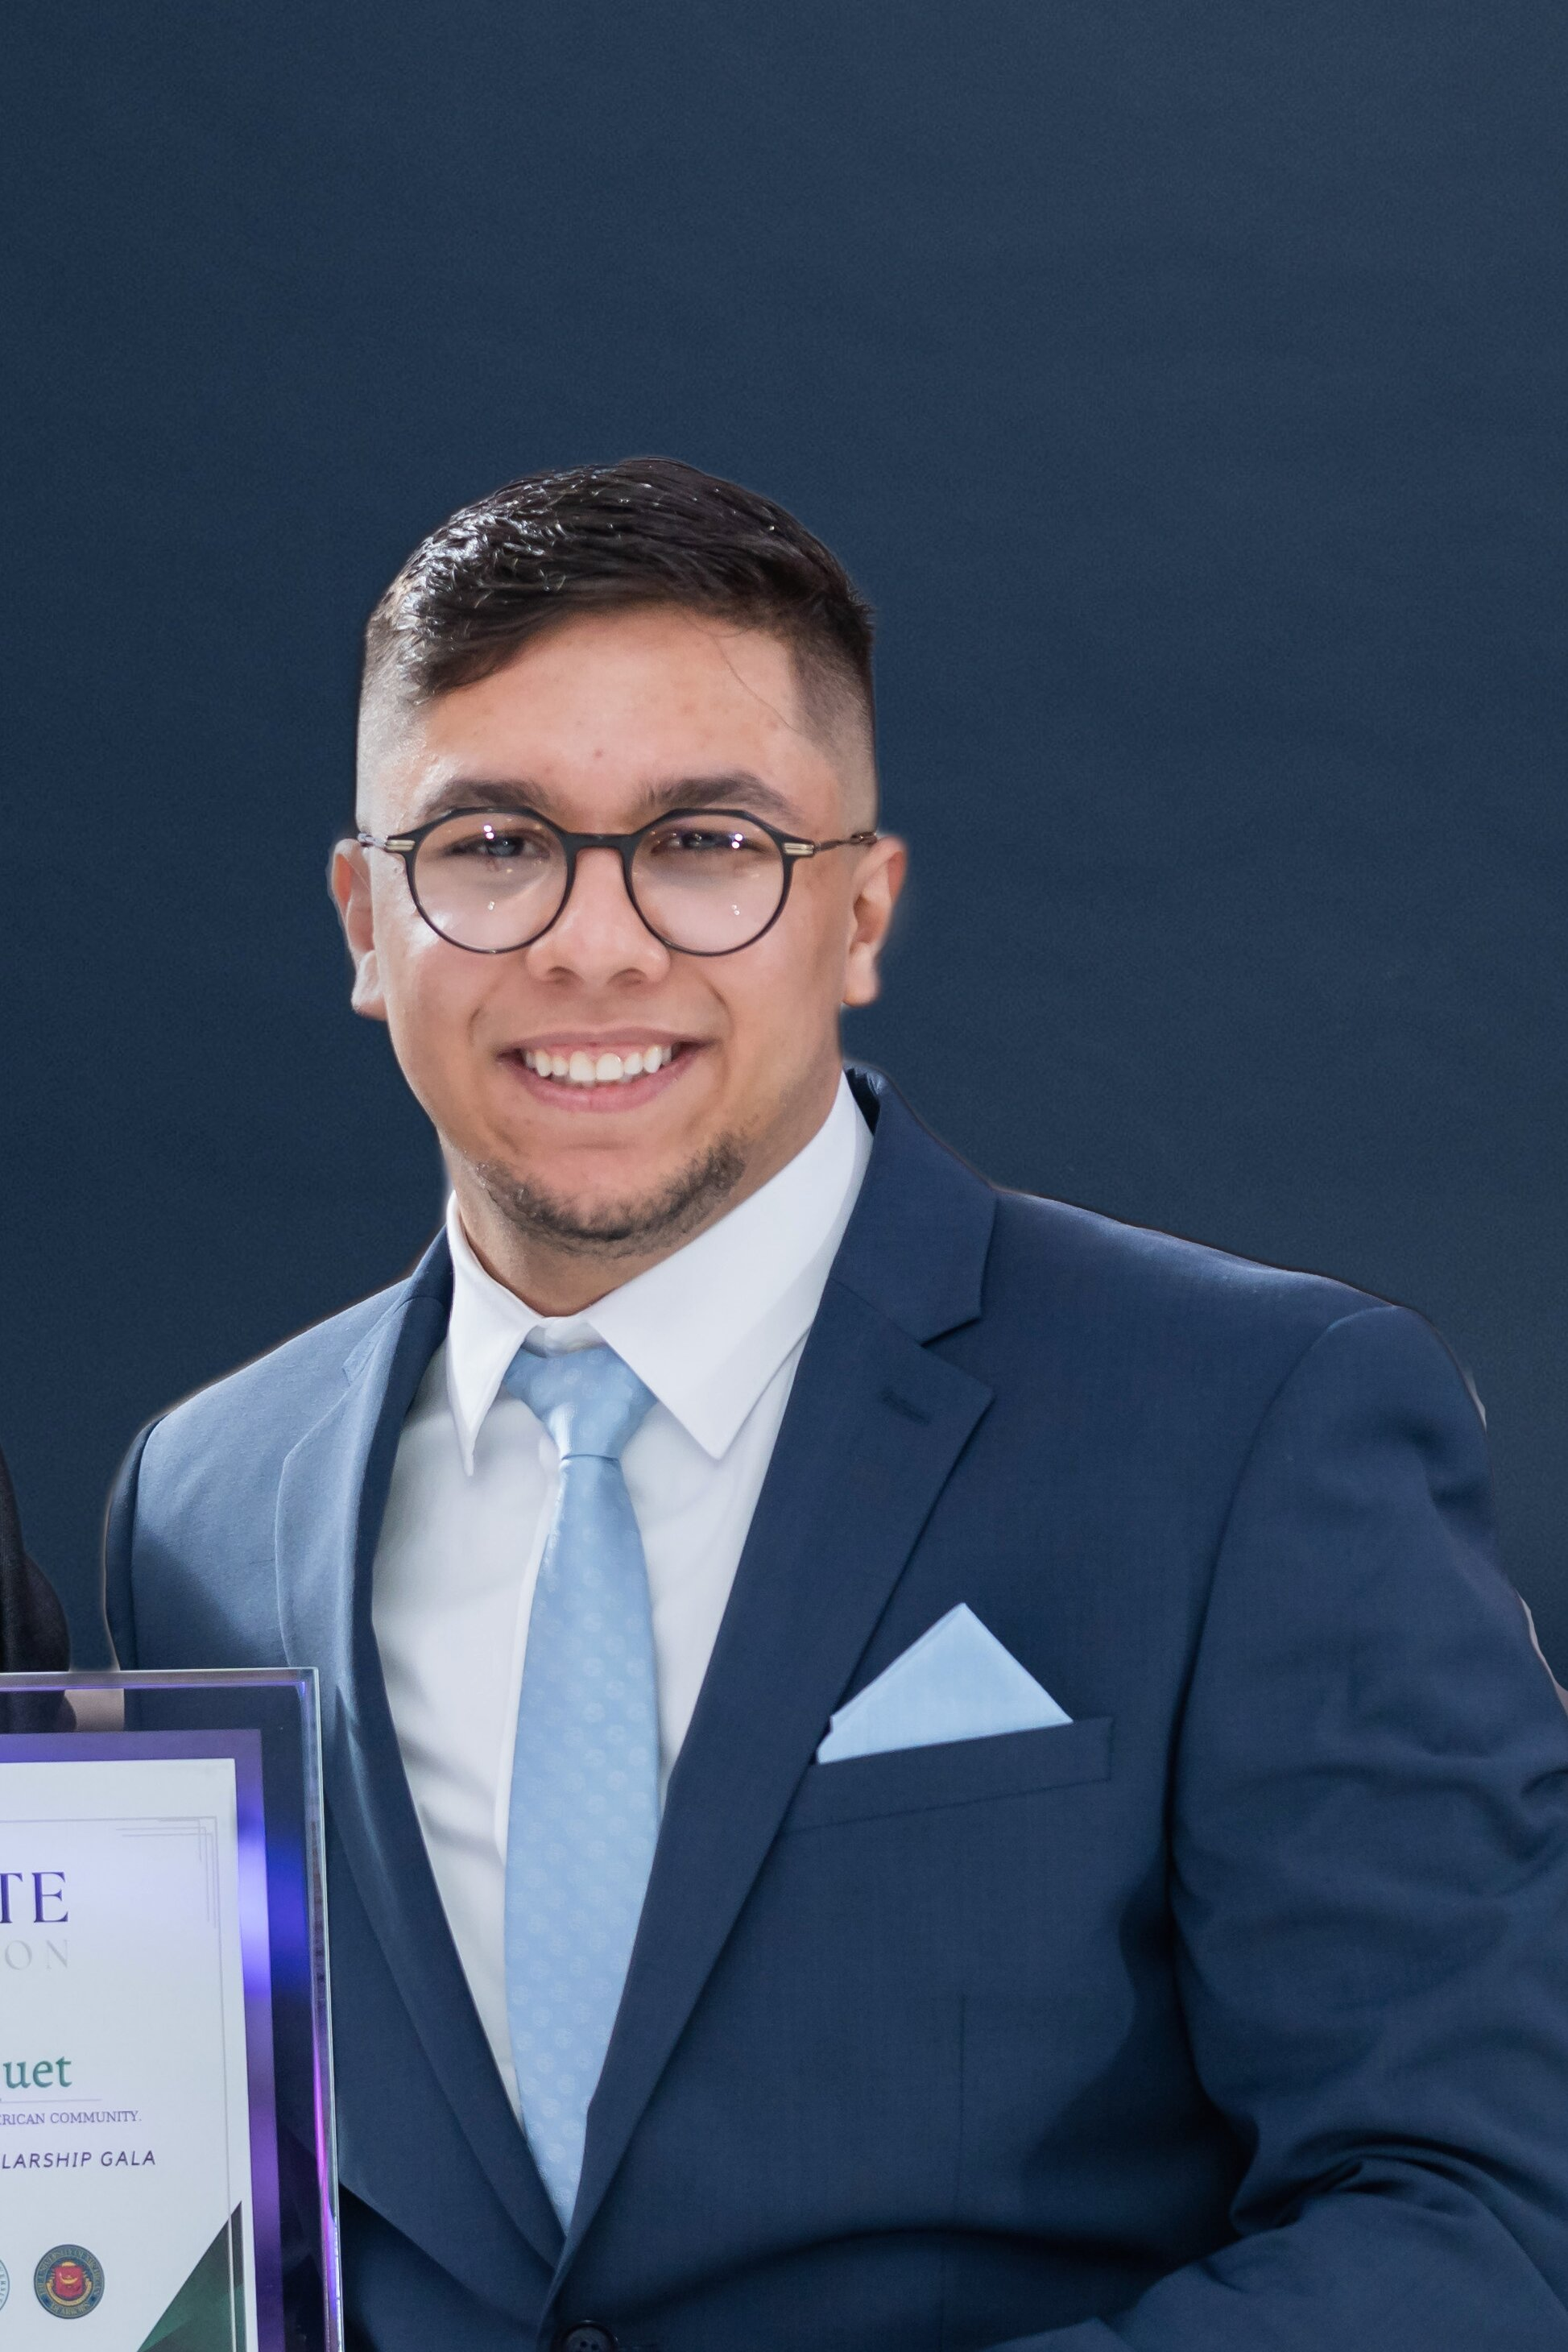
\includegraphics[width=2.38542in,height=\textheight]{Headshot.jpg}

\textbf{Background}

I was born and raised in Baghdad, Iraq, but now I live in the metro Detroit area. Besides my regular job, I love doing photography as a hobby. I enjoy capturing moments and emotions with my camera, and it lets me see the world in a whole new way. Additionally, I have a knack for analytics; I enjoy working with data, finding patterns, and gaining valuable insights from it. This analytical mindset helps me both in my photography and other aspects of life.

\textbf{Experience}

I graduated from Wayne State University in 2022 with a double major in Finance and Business Administration. For the past three years, I have been working as an IT Business Analyst at DTE Energy, where I have been involved in various analytical projects within the IT department. My responsibilities include analyzing data, identifying patterns, and providing valuable insights that contribute to the company's IT strategies and decision-making processes. I have also had the opportunity to collaborate with external consultants, showcasing my ability to work effectively with diverse teams and stakeholders. With a strong analytical mindset and a background in finance and business, I am well-equipped to contribute positively to any project or team I am a part of.

\textbf{Fun Facts}

\begin{itemize}
\item
  I am a part-time photographer, I shoot portraits, events and weddings
\item
  I enjoy playing soccer, my friends and I play twice a week
\item
  I collect vintage Ralph Lauren clothing
\end{itemize}

\hypertarget{what-is-artificial-intelligence-ai}{%
\chapter{What is Artificial Intelligence (AI)?}\label{what-is-artificial-intelligence-ai}}

Discuss what AI is here

\hypertarget{ai-tools-for-job-searching}{%
\chapter{AI Tools for Job Searching}\label{ai-tools-for-job-searching}}

\hypertarget{resume-and-cover-letter-optimizers}{%
\chapter{Resume and Cover Letter Optimizers}\label{resume-and-cover-letter-optimizers}}

\hypertarget{student-practice-interviews}{%
\chapter{Student Practice Interviews}\label{student-practice-interviews}}

\hypertarget{automated-applications}{%
\chapter{Automated Applications}\label{automated-applications}}

\hypertarget{what-are-applicant-tracking-systems-ats}{%
\chapter{What Are Applicant Tracking Systems (ATS)?}\label{what-are-applicant-tracking-systems-ats}}

\hypertarget{recruiting-chatbots}{%
\chapter{Recruiting Chatbots}\label{recruiting-chatbots}}

\hypertarget{resume-and-cover-letter-screening}{%
\chapter{Resume and Cover Letter Screening}\label{resume-and-cover-letter-screening}}

\hypertarget{video-interview-assessments}{%
\chapter{Video Interview Assessments}\label{video-interview-assessments}}

\hypertarget{skill-assessments}{%
\chapter{Skill Assessments}\label{skill-assessments}}

\hypertarget{predicting-candidates-success}{%
\chapter{Predicting Candidates' Success}\label{predicting-candidates-success}}

\hypertarget{conclusion}{%
\chapter{Conclusion}\label{conclusion}}

\hypertarget{our-working-process}{%
\chapter{Our Working Process}\label{our-working-process}}

\hypertarget{references}{%
\chapter{References}\label{references}}

  \bibliography{book.bib,packages.bib}

\end{document}
